% lualatex tenuki29
\nonstopmode


\documentclass[11pt,a4paper]{ltjsarticle}
\usepackage{listings}
\usepackage{graphicx}
\usepackage{here}
\title{手抜きについて}
\author{手抜きチーム}
\date{2019年3月25日}


\begin{document}

\maketitle

手抜きはCSAプロトコルで対局を行うコンピュータ将棋プログラムです。作者らが将棋のプログラムの仕組みを理解することを目的として開発しています。
リポジトリ:https://github.com/hikaen2/tenuki-d



\section{作者の紹介}

\subsubsection*{鈴木太朗}
鈴木はプログラマです。会社員をしています。
仕事のかたわら趣味の自転車と合唱に打ち込んでいます。
そのかたわら手抜きを作っていますが完成させる自信がありません
(夏休みの宿題を9月1日にやるタイプです)。
棋力は30級程度です。
Twitter: @hikaen2

\subsubsection*{玉川直樹}
玉川はP兼召喚士です。KPPとレーティングシステムを疑っています。将棋ウォーズ2段。
手抜きの定跡を手入力で作りました。
Twitter: @Neakih\_kick



\section{目標}


\subsection{今年の目標}

\begin{itemize}
  \item 探索をマルチスレッドにする
\end{itemize}

Ryzenを買っちゃったのでマルチスレッドにします。
これからLazy SMPを実装します。
スレッドがよくわかりません。
実装できても正しく実装できているか分からない予感がします。

\begin{itemize}
  \item KPPTで評価する
\end{itemize}

去年はなのはさんの評価バイナリでKP + PPで評価しました。
今年はAperyの評価バイナリ(大樹の枝形式)でKPPTで評価しようと思います。
Aperyの選定理由は評価バイナリがKPPTだからです。
予想として,静的評価に手番が含まれると静止探索がいらないか,もしくは軽くていいのではないかと思っています。

評価バイナリの自作については来年挑戦します。


\subsection{来年の目標}

\begin{itemize}
  \item 評価バイナリを自作する
\end{itemize}


\subsection{去年までの目標と結果}

第28回世界コンピュータ将棋選手権:
\begin{itemize}
  \item ルール通りに指す → 結果:ルール通り指した(けど千日手のチェックをしてない)
  \item 投了する(第27回では王手放置していた) → 結果:投了した。一次予選4勝4敗
  \item KPで評価する → 結果:なのはさんの評価バイナリでKP + PPで評価した
\end{itemize}

第27回世界コンピュータ将棋選手権:
\begin{itemize}
  \item 出場する → 結果:出場した
  \item 対局する → 結果:対局した。一次予選2勝5敗
\end{itemize}



\section{プログラムの構造}

この章では手抜きの構造の説明をします。


\subsection{データ構造}

盤面に81要素の1次元配列を使用しています。そのアドレッシングはこうです(図\ref{fig1}):
\begin{figure}[h]
  \centering
  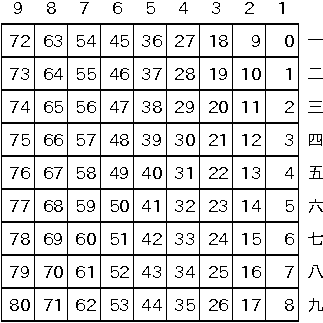
\includegraphics{fig/fig1.pdf}
  \caption{盤面のデータ構造}
  \label{fig1}
\end{figure}

第28回世界コンピュータ将棋選手権では「壁」がありましたが,なくしました。
壁がないと,壁のレイアウトを考えなくて済む,盤面がコンパクトになる,zobrist hash seedもコンパクトになる,静的評価が簡単になる(盤面のアドレッシングと評価バイナリのアドレッシングが合っていれば)といった利点があります。
一方で合法手生成が複雑になる欠点があります(1段目と9段目が繋がっているので油断すると駒がワープする)。

盤面の各要素は0から28までの値を取ります。値の意味はこうです(表\ref{tab1}のA列):
\begin{table}[h]
  \centering
  \caption{値の意味}
  \small
  \begin{tabular}{rl|llllll}
     A &        & type(A) & base(A) & color(A) & promotable(A) & promote(A) & inv(A) \\ \hline
     0 & ▲歩   & 歩   & 歩 & ▲ & T & ▲と   & △歩   \\
     1 & ▲香   & 香   & 香 & ▲ & T & ▲成香 & △香   \\
     2 & ▲桂   & 桂   & 桂 & ▲ & T & ▲成桂 & △桂   \\
     3 & ▲銀   & 銀   & 銀 & ▲ & T & ▲成銀 & △銀   \\
     4 & ▲金   & 金   & 金 & ▲ & F & ▲金   & △金   \\
     5 & ▲角   & 角   & 角 & ▲ & T & ▲馬   & △角   \\
     6 & ▲飛   & 飛   & 飛 & ▲ & T & ▲龍   & △飛   \\
     7 & ▲王   & 王   & 王 & ▲ & F & ▲王   & △王   \\
     8 & ▲と   & と   & 歩 & ▲ & F & ▲と   & △と   \\
     9 & ▲成香 & 成香 & 香 & ▲ & F & ▲成香 & △成香 \\
    10 & ▲成桂 & 成桂 & 桂 & ▲ & F & ▲成桂 & △成桂 \\
    11 & ▲成銀 & 成銀 & 銀 & ▲ & F & ▲成銀 & △成銀 \\
    12 & ▲馬   & 馬   & 角 & ▲ & F & ▲馬   & △馬   \\
    13 & ▲龍   & 龍   & 飛 & ▲ & F & ▲龍   & △龍   \\
    14 & △歩   & 歩   & 歩 & △ & T & △と   & ▲歩   \\
    15 & △香   & 香   & 香 & △ & T & △成香 & ▲香   \\
    16 & △桂   & 桂   & 桂 & △ & T & △成桂 & ▲桂   \\
    17 & △銀   & 銀   & 銀 & △ & T & △成銀 & ▲銀   \\
    18 & △金   & 金   & 金 & △ & F & △金   & ▲金   \\
    19 & △角   & 角   & 角 & △ & T & △馬   & ▲角   \\
    20 & △飛   & 飛   & 飛 & △ & T & △龍   & ▲飛   \\
    21 & △王   & 王   & 王 & △ & F & △王   & ▲王   \\
    22 & △と   & と   & 歩 & △ & F & △と   & ▲と   \\
    23 & △成香 & 成香 & 香 & △ & F & △成香 & ▲成香 \\
    24 & △成桂 & 成桂 & 桂 & △ & F & △成桂 & ▲成桂 \\
    25 & △成銀 & 成銀 & 銀 & △ & F & △成銀 & ▲成銀 \\
    26 & △馬   & 馬   & 角 & △ & F & △馬   & ▲馬   \\
    27 & △龍   & 龍   & 飛 & △ & F & △龍   & ▲龍   \\
    28 & 空     & 空   & 空 & -  & F & 空     & 空
  \end{tabular}
  \label{tab1}
\end{table}

第28回世界コンピュータ将棋選手権では手番と成りをビット演算で管理していましたが,表で管理するようにしました。
表で管理するとビットレイアウトを考えなくて済む利点があります。
一方,表を引くのに(ビット演算よりは)時間がかかる欠点がありそうです。

表のtype(A)の列からinv(A)の列まではA列の関数です。
意味はこうです:
\begin{itemize}
  \item type(A): Aから手番を除いた値
  \item base(A): Aから手番を除いて成りを戻した値。駒を取ったときに使う。
  \item color(A): Aの手番
  \item promotable(A): Aが成れる駒かどうか
  \item promote(A): Aが成った駒
  \item inv(A): Aの手番を反転した駒
\end{itemize}

こうして見ると全部で6つもあって多いように思います。
全部で4つくらいになってもいいような気がします。


\subsection{探索}

mini-max探索をしています。

\begin{itemize}
  \item αβ枝刈りをしています。最近やっとαβ枝刈りが何なのか分かるようになりました。
  \item null-move枝刈りをしています。
  \item 静止探索しています。
  \item 指し手だけの置換表(指し手表?)があります。表のエントリは指し手だけです。
  一般的な置換表のエントリにはミスヒット検出のために局面のハッシュ値が入れてありますが,手抜きでは入れていません。
  指し手だけの表なのでミスヒットしても害がないと考えているためです。しかしLazy SMPしはじめると問題があるかもしれません。
  \item Lazy SMPしたいです。
  \item futility枝刈りしていません。静的評価が差分評価でないからです。
\end{itemize}


\subsection{静的評価}

Apery, commit 3221627(2016年11月3日)の評価バイナリを使ってKPPTで評価する予定です。
以下はAperyの評価バイナリについての覚書です(独自調査;間違ってたらすみません)。

\subsubsection*{覚書}
Aperyはcommit a0a09de(2015年10月15日)で手番評価を実装しKPPT評価になった(それ以前はKPP評価だった)。その評価バイナリには以下の3つのファイルがある:

\begin{itemize}
  \item KK\_synthesized.bin(52,488バイト)
  \item KKP\_synthesized.bin(81,251,424バイト)
  \item KPP\_synthesized.bin(776,402,496バイト)
\end{itemize}

それぞれのファイルには,通常の評価値と手番を持つ側に加算される評価値の2つ組が,複数個格納されている\footnote{NineDayFever http://www2.computer-shogi.org/wcsc24/appeal/NineDayFever/NDF.txt}。
それぞれの評価値は2バイトもしくは4バイトの符号付き整数でリトルエンディアンである。

KK\_synthesized.binには4バイトの評価値を持つ2つ組(8バイト)が81(先手玉の位置) \times 81(後手玉の位置) = 6,561個格納されている。

KKP\_synthesized.binには4バイトの評価値を持つ2つ組(8バイト)が81(先手玉の位置) \times 81(後手玉の位置) \times 1548(※) = 10,156,428個格納されている。

KPP\_synthesized.binには2バイトの評価値を持つ2つ組(4バイト)が81(自玉の位置) \times 1548(※) \times 1548(※) = 194,100,624個格納されている。\\

※:表\ref{tab2}の1548要素。\\

\begin{table}[h]
  \centering
  \caption{1548要素の内訳}
  \small
  \begin{tabular}{lrrr}
    内容 & from & to & 要素数 \\ \hline
    味方の持駒の歩の0枚目~18枚目の評価値 &  0 & 18 & 19 \\
    相手の持駒の歩の0枚目~18枚目の評価値 & 19 & 37 & 19 \\
    味方の持駒の香の0枚目~4枚目の評価値  & 38 & 42 &  5 \\
    相手の持駒の香の0枚目~4枚目の評価値  & 43 & 47 &  5 \\
    味方の持駒の桂の0枚目~4枚目の評価値  & 48 & 52 &  5 \\
    相手の持駒の桂の0枚目~4枚目の評価値  & 53 & 57 &  5 \\
    味方の持駒の銀の0枚目~4枚目の評価値  & 58 & 62 &  5 \\
    相手の持駒の銀の0枚目~4枚目の評価値  & 63 & 67 &  5 \\
    味方の持駒の金の0枚目~4枚目の評価値  & 68 & 72 &  5 \\
    相手の持駒の金の0枚目~4枚目の評価値  & 73 & 77 &  5 \\
    味方の持駒の角の0枚目~2枚目の評価値  & 78 & 80 &  3 \\
    相手の持駒の角の0枚目~2枚目の評価値  & 81 & 83 &  3 \\
    味方の持駒の飛の0枚目~2枚目の評価値  & 84 & 86 &  3 \\
    相手の持駒の飛の0枚目~2枚目の評価値  & 87 & 89 &  3 \\
    味方の歩がアドレス0~80にいるときの評価値 &   90 &  170 & 81 \\
    相手の歩がアドレス0~80にいるときの評価値 &  171 &  251 & 81 \\
    味方の香がアドレス9~80にいるときの評価値 &  252 &  332 & 81 \\
    相手の香がアドレス0~80にいるときの評価値 &  333 &  413 & 81 \\
    味方の桂がアドレス0~80にいるときの評価値 &  414 &  494 & 81 \\
    相手の桂がアドレス0~80にいるときの評価値 &  495 &  575 & 81 \\
    味方の銀がアドレス0~80にいるときの評価値 &  576 &  656 & 81 \\
    相手の銀がアドレス0~80にいるときの評価値 &  657 &  737 & 81 \\
    味方の金がアドレス0~80にいるときの評価値 &  738 &  818 & 81 \\
    相手の金がアドレス0~80にいるときの評価値 &  819 &  899 & 81 \\
    味方の角がアドレス0~80にいるときの評価値 &  900 &  980 & 81 \\
    相手の角がアドレス0~80にいるときの評価値 &  981 & 1061 & 81 \\
    味方の馬がアドレス0~80にいるときの評価値 & 1062 & 1142 & 81 \\
    相手の馬がアドレス0~80にいるときの評価値 & 1143 & 1223 & 81 \\
    味方の飛がアドレス0~80にいるときの評価値 & 1224 & 1304 & 81 \\
    相手の飛がアドレス0~80にいるときの評価値 & 1305 & 1385 & 81 \\
    味方の龍がアドレス0~80にいるときの評価値 & 1386 & 1466 & 81 \\
    相手の龍がアドレス0~80にいるときの評価値 & 1467 & 1547 & 81 \\ \hline
                                              &      & 合計: & 1548
  \end{tabular}
  \label{tab2}
\end{table}

例:
\begin{enumerate}
  \small
  \item KK[44][36][0] : 先手玉がアドレス44にいて,後手玉がアドレス36にいるときの評価値
  \item KK[44][36][1] : 先手玉がアドレス44にいて,後手玉がアドレス36にいるときの,手番を持つ側に加算される評価値
  \item KKP[44][36][1][0] : 先手玉がアドレス44にいて,後手玉がアドレス36にいるときの,先手の持駒の1枚目の歩の評価値
  \item KKP[44][36][1][1] : 先手玉がアドレス44にいて,後手玉がアドレス36にいるときの,先手の持駒の1枚目の歩の,手番を持つ側に加算される評価値
  \item KKP[44][36][2][0] : 先手玉がアドレス44にいて,後手玉がアドレス36にいるときの,先手の持駒の2枚目の歩の評価値
  \item KKP[44][36][20][0] : 先手玉がアドレス44にいて,後手玉がアドレス36にいるときの,後手の持駒の1枚目の歩の評価値
  \item KKP[44][36][576][0] : 先手玉がアドレス44にいて,後手玉がアドレス36にいるときの,アドレス0にいる先手の銀の評価値
  \item KKP[44][36][657][0] : 先手玉がアドレス44にいて,後手玉がアドレス36にいるときの,アドレス0にいる後手の銀の評価値
  \item KPP[44][1][2][0] : 自玉がアドレス44にいるときに,味方の持駒の1枚目の歩から見た,味方の持駒の2枚目の歩の評価値
  \item KPP[44][1][2][1] : 自玉がアドレス44にいるときに,味方の持駒の1枚目の歩から見た,味方の持駒の2枚目の歩の,手番を持つ側に加算される評価値
  \item KPP[44][1][20][0] : 自玉がアドレス44にいるときに,味方の持駒の1枚目の歩から見た,相手の持駒の1枚目の歩の評価値
  \item KPP[44][1][2][576] : 自玉がアドレス44にいるときに,味方の持駒の1枚目の歩から見た,アドレス0にいる味方の銀の評価値
  \item KPP[44][1][2][657] : 自玉がアドレス44にいるときに,味方の持駒の1枚目の歩から見た,アドレス0にいる相手の銀の評価値
  \item KPP[44][576][577][0] : 自玉がアドレス44にいるときに,アドレス0にいる味方の銀から見た,アドレス1にいる味方の銀の評価値
  \item KPP[44][576][658][0] : 自玉がアドレス44にいるときに,アドレス0にいる味方の銀から見た,アドレス1にいる相手の銀の評価値
\end{enumerate}


\end{document}
